% hello.tex - Our first LaTeX example!

\documentclass{article}
\usepackage{graphicx}
\usepackage[top=2.54cm, bottom=2.54cm, left=1.25cm, right=1.25cm]{geometry}
\usepackage{mathtools}
\DeclarePairedDelimiter{\abs}{\lvert}{\rvert}
\usepackage{enumerate}
\usepackage{url}


\begin{document}

\title{Foosball: CS296 Project, Group 27}

\author{
Kiran Y - 120050049,\\
\texttt{120050049@iitb.ac.in,}\\
Mihir -12D020007\\
\texttt{mihirk.1994@iitb.ac.in}\\
Harinandan Teja-120050066\\
\texttt{120050066@iitb.ac.in}\\
}
\date{\today}

\maketitle

\section{Introduction}
This report explains in detail the project we created- a foosball table- in Box2d. We describe in brief the bodies,fixtures and constraints we used to create this simulation.\\
Here is the initial model of our simulatiom:
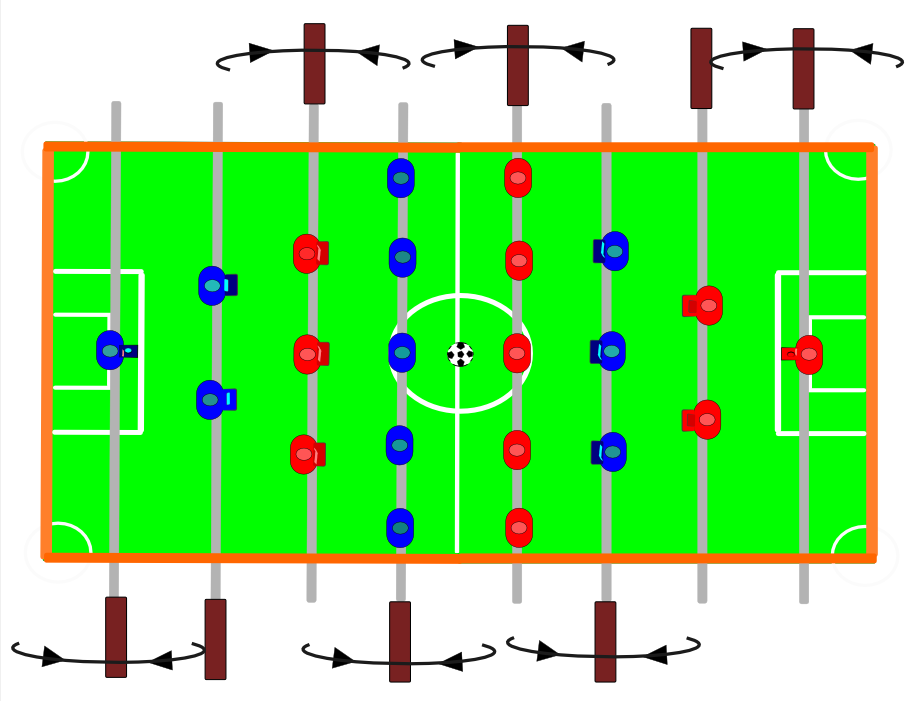
\includegraphics[width=100pt,height=100pt]{foosball}
\section{Parts of the simulation}

\subsection{Table}
The entire game is played within the confines of the table, which serves to restrict the motion of the ball and rods. This was implemented using four box shapes.\\
\includegraphics[width=100pt,height=100pt]{Platform}

\subsection{Rods}
This is a new sphere, identical in shape to the old heavy sphere but much lighter. It rests on the new horizontal platform and is knocked ahead by the light box, after which it collides with the dominoes and goes into the new box.\\

\includegraphics[width=100pt,height=100pt]{Newsphere}\\

By the Law of Conservation of momentum \cite{resnick}
\begin{eqnarray}
M{u_x} = M{u'_x} + m{v_x} \label {eq1:simp}
\end {eqnarray}
where \\\\
$M$ : Mass of light box ($kg$)\\
$m$ : Mass of New Sphere($kg$)\\
$u_x$ : X-velocity of light box before collision ($m/s$) \\
${v_x}$ : X-velocity of light box after collision ($m/s$)\\
${u'_x}$ : X-velocity of New Sphere after collision ($m/s$)\\


\subsection{New Dominoes}
These are a set of seven new dominoes placed on the horizontal platform. The first one is knocked over by the New Sphere and it sets of a chain of dominoes knocking over their neighbour. Finally, all of them fall into the new box.\\

\includegraphics[width=100pt,height=100pt]{Dominos}\\

This is governed by the equations \cite{resnick} \\

\begin{eqnarray}
m_1\vec{v_1} + m_2\vec{v_2} = m_1\vec{v_1'} + m_2\vec{v_2'} \label  {eq2:simp} \\
\frac{1}{2}m_1\abs{\vec{v_1}}^2 + \frac{1}{2}m_1\abs{{\vec{v_1}}}^{2} = \frac{1}{2}m_1{\abs{\vec{v_1}}^{2}} + \frac{1}{2}m_1{\abs{\vec{v_1}}^{2}} \label  {eq3:simp}
\end{eqnarray}

where \\\\
$m_1$ : Mass of domino ($kg$)\\
$m_2$ : Mass of New Sphere/adjacent domino ($kg$)\\
$\vec{v_1}$ : Velocity vector of domino before collision ($m/s$) \\
$\vec{v_2}$ : Velocity vector of new sphere/adjacent domino before collision ($m/s$)\\
$\vec{v_1'}$ : Velocity vector of domino after collision ($m/s$)\\
$\vec{v_2'}$ : Velocity vector of new sphere/adjacent domino after collision ($m/s$)\\


\subsection{New Box}
This is a new box into which the New Sphere and the New Dominoes fall at the end of the animation. It is unsymmetric so as to prevent the new sphere from bouncing out.The ball bounces off the walls a couple of times before finally settling down.\\

\includegraphics[width=100pt,height=100pt]{Newbox} \\

The ball has a series of inelastic collisions with the walls of the box. The equations governing each such collison are:

\begin{eqnarray}
eu_{\perp} = {v_{\perp}} \label {eq4:simp} \\
{u_{\parallel}} = {v_{\parallel}} \label {eq5:simp}
\end{eqnarray}
\\
\\
$e$: Coefficient of restitution \\ 
${u_{\perp}}$: Initial velocity of ball perpendicular to wall($m/s$) \\ 
${v_{\perp}}$: Final velocity of ball perpendicular to wall($m/s$) \\ 
${u_{\parallel}}$: Initial velocity of ball parallel to wall($m/s$) \\ 
$v_{\parallel}$: Final velocity of ball parallel to wall($m/s$) \\ 


\section{Conclusion}
The simulation is identical to the old one for the intial part. When the light box flies up into the air, it knocks the new sphere onto the dominoes and all of them fall down into a new box. The old sphere comes to rest near the wall of the new box. The rest of the animation is unchanged\\
In conclusion, we have added a few features to the simulation to make it more interesting while conserving its basic functionality \\
\bibliographystyle{plain}
\bibliography{cs296_report_27}

\end{document}
